\section{pbdR}

\hidenum
\begin{frame}[noframenumbering]
\frametitle{Contents}
 \tableofcontents[currentsection,hideothersubsections,sectionstyle=show/hide]
\end{frame}
\shownum


\subsection{The pbdR Project}


\begin{frame}
  \begin{block}{Programming with Big Data in R (pbdR)}
       \centering Striving for \emph{Productivity, Portability, Performance}\\[.4cm]\pause
  \begin{columns}[onlytextwidth]
    \begin{column}{0.30\textwidth}
      \centering
       
\includegraphics[width=3.4cm]{../common/pics/simple}\\[.2cm]
    \end{column}
    \begin{column}{0.65\textwidth}
  \begin{itemize}[<+-|alert@+>]
    \item \emph{Free}\footnote{MPL, BSD, and GPL licensed} R packages.
    \item Bridging high-performance C with high-productivity of R
    \item Scalable, big data analytics.
    \item Distributed data details implicitly managed.
    \item Methods have syntax \emph{identical} to R.
    \item Powered by state of the art numerical libraries (MPI, ScaLAPACK, \dots)
  \end{itemize}
    \end{column}
​  \end{columns}
\end{block}
\end{frame}




\begin{frame}
  \begin{block}{pbdR Packages}
    \begin{center}
%         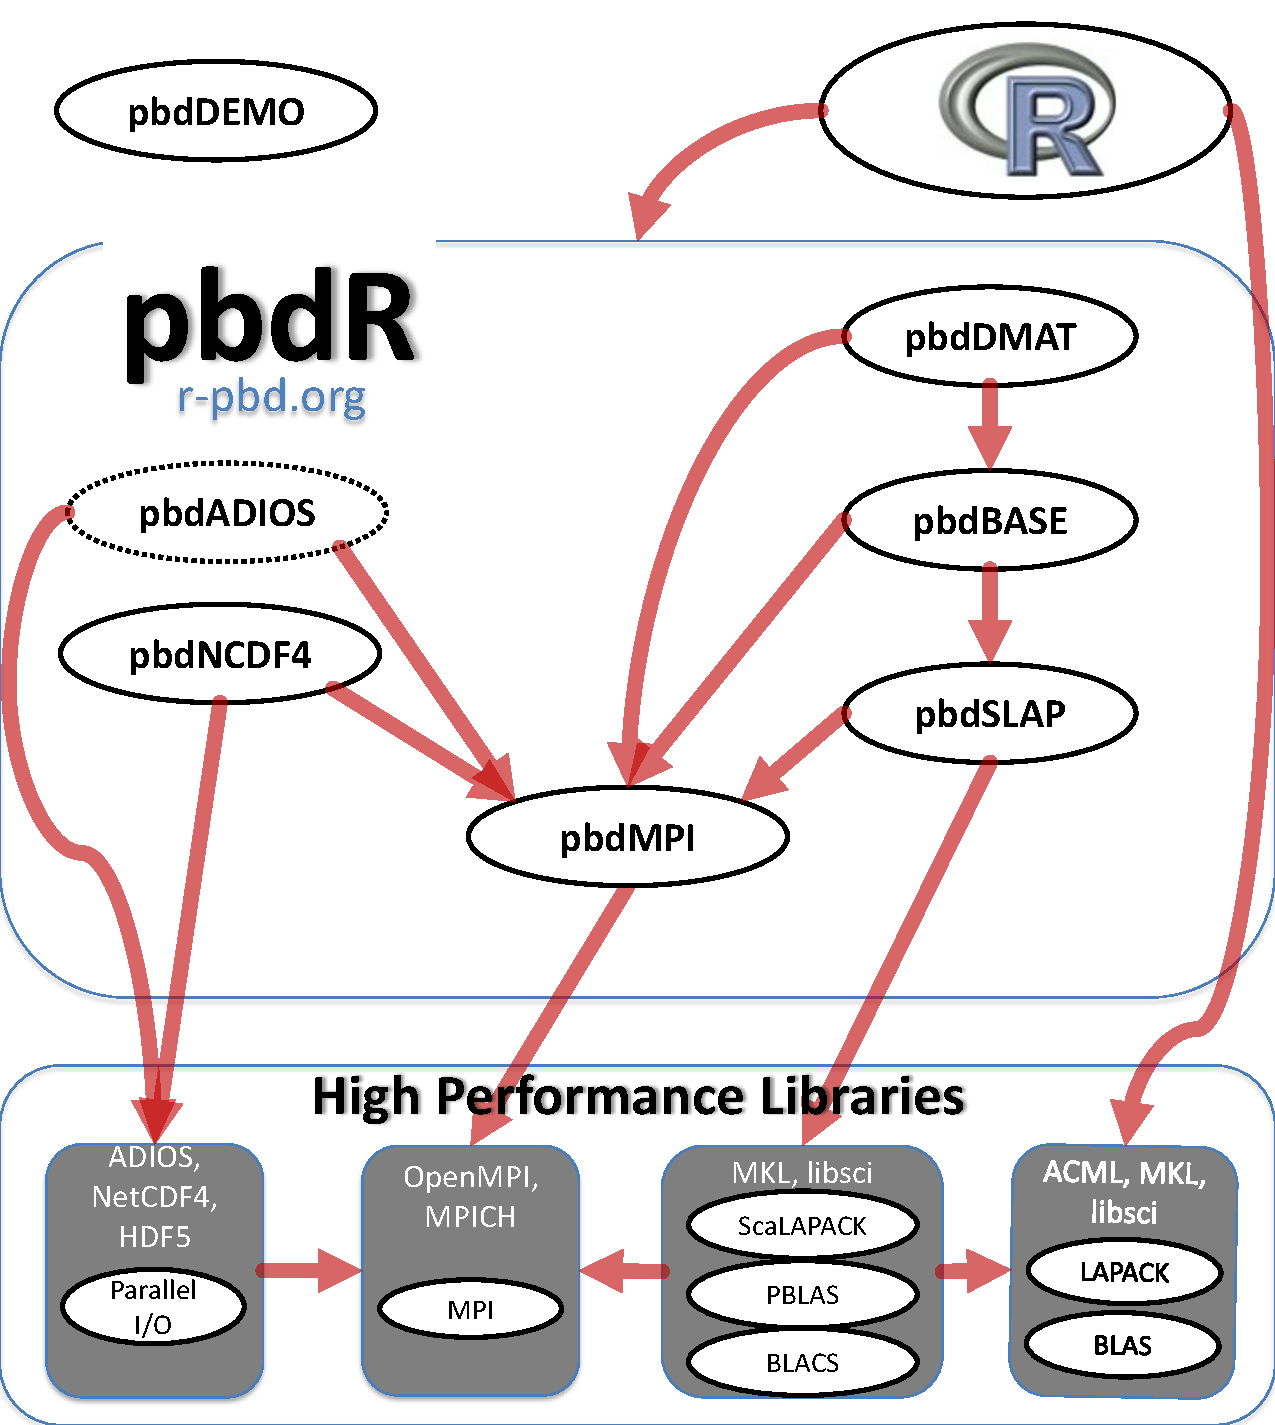
\includegraphics[width=7cm, height=7cm]{pics/pbdpacks}
      \begin{columns}
        \begin{column}{.52\textwidth}
      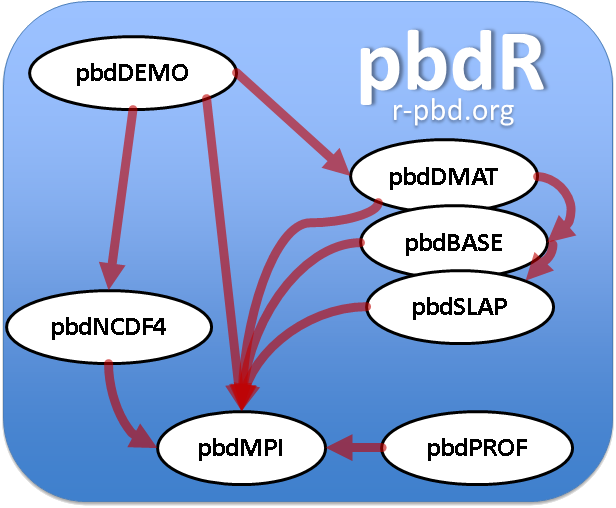
\includegraphics[scale=.4]{../common/pics/pbdR}
        \end{column}
        \hfill
        \begin{column}{.4\textwidth}
      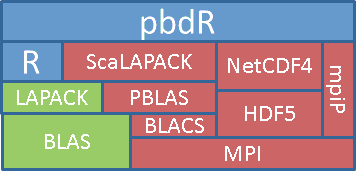
\includegraphics[scale=.45]{../common/pics/libs}
        \end{column}
      \end{columns}
    \end{center}
  \end{block}
\end{frame}


% \begin{frame}[shrink]
%   \begin{block}{pbdR Packages --- http://code.r-pbd.org}\pause
%   Released to CRAN:
%   \begin{itemize}[<+-|alert@+>]
%     \item \pkg{pbdMPI}: MPI bindings (explicit, low-level)
%     \item \pkg{pbdSLAP}: Foreign library (just install it, nothing to use)
%     \item \pkg{pbdBASE}: Compiled code (used by DMAT, also for devs)
%     \item \pkg{pbdDMAT}: Distributed matrices (mostly implicit, high-level)
%     \item \pkg{pbdNCDF4}: Parallel NetCDF4 reader
%     \item \pkg{pbdDEMO}: Package demonstrations, examples, vignette written in textbook style
%     \item \pkg{pmclust}: Parallel model-based clustering.
%   \end{itemize}
% %     \\[.2cm]
%     Future Development:
%   \begin{itemize}[<+-|alert@+>]
%     \item Updates and expansions
%     \item \href{http://rwiki.sciviews.org/doku.php?id=developers:projects:gsoc2013:mpiprofiler}{Profiling Tools for Parallel Computing with R}
%     \item \dots
%   \end{itemize}
%   \end{block}
% \end{frame}


\begin{frame}[fragile]
  \begin{block}{Example Syntax}\pause
  \begin{lstlisting}
x <- x[-1, 2:5]
x <- log(abs(x) + 1)
xtx <- t(x) %*% x
ans <- svd(solve(xtx))
  \end{lstlisting}
  \begin{center}
  \pause Look familiar?\\[.4cm] \pause
  \emph{The above runs on 1 core with R or 10,000 cores with pbdR}
  \end{center}
  \end{block}
\end{frame}


\begin{frame}
  \begin{block}{Least Squares Benchmark}\pause
  \begin{center}
  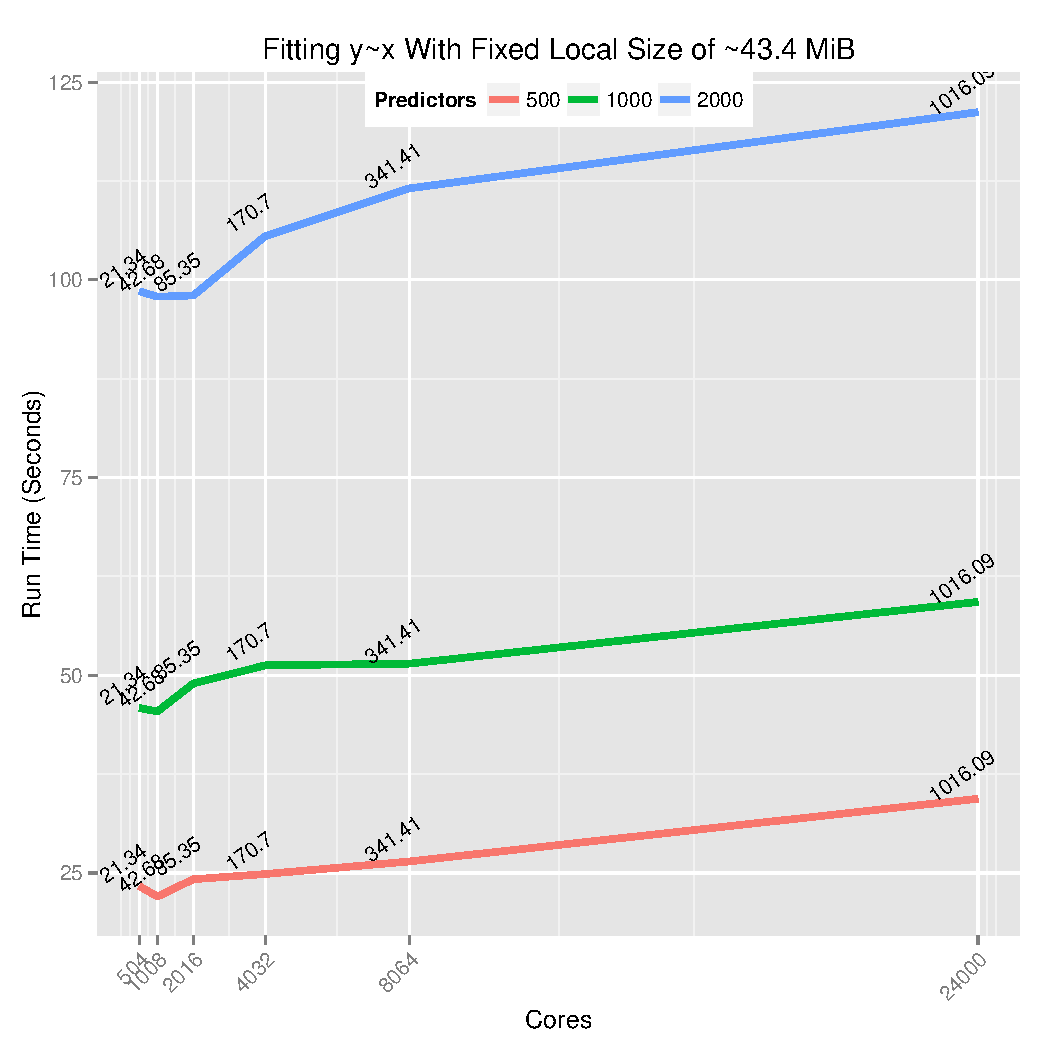
\includegraphics[height=.89\textheight]{../common/pics/lmfit2}
  \end{center}
  \end{block}
\end{frame}

\begin{frame}[fragile]
  \begin{block}{Profiling with \textbf{pbdPROF}}
  \begin{minipage}[t]{.58\textwidth}
  \vspace{0pt}
  1. Rebuild \pbdR\ packages
\vspace*{-.5cm}
\begin{lstlisting}[language=shl,title=\ ]
R CMD INSTALL pbdMPI_0.2-1.tar.gz \ --configure-args= \ "--enable-pbdPROF"
\end{lstlisting}
2. Run code
\vspace*{-.5cm}
\begin{lstlisting}[language=shl,title=\ ]
mpirun -np 64 Rscript my_script.R
\end{lstlisting}

3. Analyze results
\vspace{-.5cm}
\begin{lstlisting}[title=\ ]
library(pbdPROF)
prof <- read.prof( "profiler_output.mpiP")
plot(prof)
\end{lstlisting}
  \end{minipage}
  \hfill
  \begin{minipage}[t]{.4\textwidth}
  \vspace{0pt}
    \centering
    Publication-quality graphs\\
    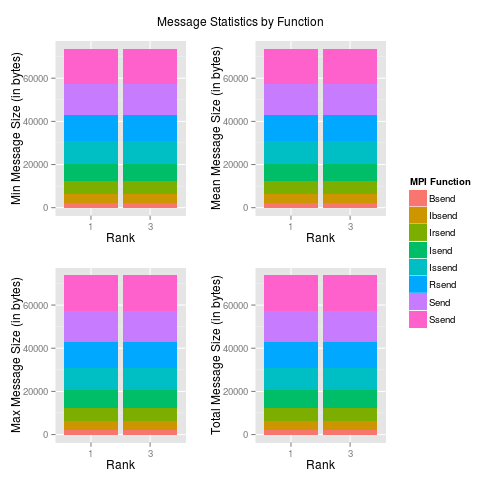
\includegraphics[scale=.25]{pics/mpip}
    \\[.1cm]
    
\includegraphics[scale=0.3]{pics/gsoc}
  \end{minipage}
  \end{block}
\end{frame}




\subsection{pbdR Paradigms}

\begin{frame}
  \begin{block}{pbdR Paradigms}
  Programs that use pbdR utilize:
  \begin{itemize}[<+-|alert@+>]
   \item Batch execution
   \item Single Program/Multiple Data (SPMD) style
%    \item Object Oriented Programming (OOP)
   \\[.2cm]
   \end{itemize}
    And generally utilize:
   \begin{itemize}
   \item Data Parallelism
  \end{itemize}
  \end{block}
\end{frame}


\begin{frame}[fragile]
  \begin{block}{Batch Execution}\pause
    \begin{itemize}
      \item Non-interactive
      \item Use
\vspace{-.4cm}
\begin{lstlisting}[language=sh]
Rscript my_script.r
\end{lstlisting}
or\vspace{-.4cm}
\begin{lstlisting}[language=sh]
R CMD BATCH my_script.r
\end{lstlisting}
      \item In parallel:
\vspace{-.4cm}
\begin{lstlisting}[language=sh]
mpirun -np 2 Rscript my_par_script.r
\end{lstlisting}
    \end{itemize}
  \end{block}
\end{frame}


\begin{frame}
  \begin{block}{Single Program/Multiple Data (SPMD)}\pause
    \begin{itemize}
      \item SPMD is a programming \emph{paradigm}.
      \item Not to be confused with SIMD.
      \item SPMD utilizes MIMD architecture computers.
      \item Arguably the simplest extension of serial programming.
    \end{itemize}
  \end{block}
\end{frame}


\begin{frame}
  \begin{block}{Single Program/Multiple Data (SPMD)}\pause
    \begin{itemize}
      \item Difficult to describe, easy to do\dots
      \item Only one program is written, executed in batch on all processors.
      \item Different processors are autonomous; there is no manager.
      \item The dominant programming model for large machines.
    \end{itemize}
  \end{block}
\end{frame}


\begin{frame}[fragile]
  \begin{block}{SPMD}
    \begin{center}
%       \begin{columns}
        \begin{minipage}{.47\textwidth}
        \begin{block}{Manager/Worker}
        \begin{itemize}
          \item Fascism
          \item Resentment
          \item Fealty
        \end{itemize}
        \end{block}
        \end{minipage}
        %
        \hspace{.1cm}
        %
        \begin{minipage}{.47\textwidth}
        \begin{block}{SPMD}
        \begin{itemize}
          \item Democracy
          \item Cooperation
          \item Freeedom
        \end{itemize}
        \end{block}
        \end{minipage}
%       \end{columns}
    \end{center}
  \end{block}
\end{frame}


% \begin{frame}
%   \begin{block}{Manager/Worker vs SPMD}
%    \begin{center}
%    Graphics will go here\\
%     \begin{minipage}[t]{.47\textwidth}
%     \begin{block}{\centering Manager/Worker:  Fascism}
% %image
%     \end{block}
%     \end{minipage}
%     \hspace{.1cm}
%     \begin{minipage}[t]{.47\textwidth}
%     \begin{block}{\centering SPMD: Democracy}
% %image 
%     \end{block}
%     \end{minipage}
%     \end{center}
%     \end{block}
% \end{frame}